
\documentclass{cmc}


\begin{document}

\pagestyle{fancy}
\lhead{\textit{\textbf{Computational Motor Control, Spring 2018} \\
    Python exercise, Lab 4, GRADED}} \rhead{Student \\ Names}

\section*{Student names: \ldots (please update)}

\textit{Instructions: Update this file (or recreate a similar one,
  e.g.\ in Word) to prepare your answers to the questions. Feel free
  to add text, equations and figures as needed. Hand-written notes,
  e.g.\ for the development of equations, can also be included e.g.\
  as pictures (from your cell phone or from a scanner).
  \textbf{\corr{This lab is graded.}} and need to be submitted before
  the \textbf{\corr{Deadline : 03-04-2018 Midnight}}.  \\ Please
  submit both the source file (*.doc/*.tex) and a pdf of your
  document, as well as all the used and updated Python functions in a
  single zipped file called \corr{lab4\_name1\_name2\_name3.zip} where
  name\# are the team member’s last names.  \corr{Please submit only
    one report per team!}}

\textit{In this exercise, you will explore the different modelling
  techniques that can be used to control a single joint and
  segment. We initially start by exploring a single joint controlled
  by a pair of antagonist spring like muscles and then extend the
  model by adding dampers to it. These only represent the passive
  dynamics observed in a real musculoskeletal system. To make the
  behaviour more realistic we then study more complex hill muscle
  model in detail. }

\section*{Exercise 1 : Pendulum model with passive elements}
\label{sec:question-1}

Mechanical behavior of muscle tissue can be described by simple
passive elements such as springs and dampers. These elements, when
combined properly, allow to study the behavior of muscle under
compressive and tensile loads.

\subsection*{Explore the pendulum model with two antagonist spring
  elements}

In this question the goal is to add two antagonist springs to the
pendulum model which you are already familiar with from lab 2
exercises. For simplicity we assume the springs directly apply a
torsional force on to the pendulum.  Use equation \ref{eqn:spring} to
develop the spring model.

\textit{\textbf{Note} : The springs can only produce force in
  one-direction like the muscles.  That is, they can only apply a
  pulling force and apply a zero force when compressed.  You need to
  accomodate for this condition for springs S1 and S2 in the equation
  shown below}

The setup for the pendulum with a pair of antagonist springs is as
shown in figure \ref{fig:pendulum_spring}. Use \fileref{exercise1.py},
\fileref{lab4\_pendulum.py} and \fileref{SystemParameters.py} files to
complete the exercise.

\begin{equation}
  \label{eqn:spring}
  F_{s} = K*(\theta_{ref} - \theta)
\end{equation}

Where,
\begin{itemize}
\item $F_{s}$ : Torsional Spring force
\item $K$ : Spring Constant
\item $\theta_{ref}$ : Spring reference angle
\item $\theta$ : pendulum angle
\end{itemize}


\begin{figure}[H]
  \centering
  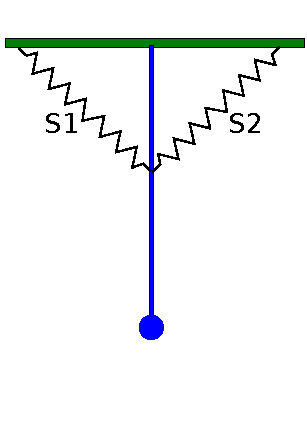
\includegraphics[width=.3\textwidth]{figures/pendulum_spring}
  \caption[pendulum with spring]{Pendulum model with two springs s1
    and s2}
  \label{fig:pendulum_spring}
\end{figure}


\subsection*{1.a Does the system have a stable limit cycle behavior?
  Describe and run an experiment to support your answer.}
\label{subsec:1.a}



\subsection*{1.b Explore the role of spring constant ($K$) and spring
  reference angle ($\theta_0$) in terms of range of motion, amplitude,
  ... \\ Support your responses with relevant plots }


\subsection*{1.c Explain the behavior of the model when you have
  different spring constants ($K$) and spring reference angles
  ($\theta_{ref}$). Support your responses with relevant plots}

\subsection*{Explore the pendulum model with two antagonist spring and damper elements}
Over time muscles lose energy while doing work. In order to account
for this property, let us now add a damper in parallel to the spring
model. Use equation \ref{eqn:damper} to develop the damper model.

\textit{\textbf{Note} : Like the previous springs, dampers can only
  produce force in one-direction.  That is, they can only apply a
  damping force in the pulling direction and apply a zero force when
  compressed. You need to accomodate for this condition for dampers B1
  and B2 in the equation shown below}

Again use \fileref{exercise1.py}, \fileref{lab4\_pendulum.py} and
\fileref{SystemParameters.py} files to complete the exercise. The
setup for the pendulum model with a pair of antagonist spring and
dampers in parallel is as shown in figure
\ref{fig:pendulum_spring_damper}.


\begin{equation}
  \label{eqn:damper}
  F_{B} = B*(\dot{\theta})
\end{equation}

Where,
\begin{itemize}
\item $F_{B}$ : Torsional Damper force
\item $B$ : Damping Constant
\item $\dot{\theta}$ : pendulum angular velocity
\end{itemize}


\begin{figure}[H]
  \centering
  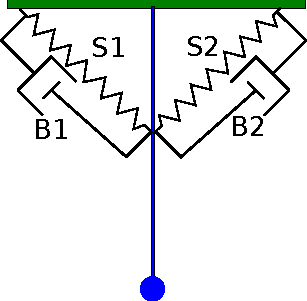
\includegraphics[width=.3\textwidth]{figures/pendulum_spring_damper}
  \caption[pendulum with spring]{Pendulum model with two springs S1
    and S2 and two dampers B1 and B2}
  \label{fig:pendulum_spring_damper}
\end{figure}


\subsection*{1.d How does the behavior now change compared to
  1.a. Briefly explain and support your responses with relevant plots}

\subsection*{1.e Can you find a combination of spring constant ($K$),
  damping constant ($B$) and spring reference angle ($\theta_{ref}$) that
  makes the pendulum rest in a stable equilibrium at
  ($\theta = \pi/6$) radians? Describe the parameters used and support
  your response with relevant plots.}

\subsection*{1.f What is the missing component between a real muscle
  and the muscle model with passive components that you just
  explored? What behaviour's do you lack because of this missing component?}


\newpage
\section*{Exercise 2 : Hill muscle model}
\label{sec:question-2}

In exercise 1, you explored the role of different passive components
and the effects of its parameters on the system. In this exercise, we
try to understand the contractile or the active element of the hill
muscle model. The components of the hill muscle are described in
figure \ref{fig:hill_muscle}. The equations used to model the hill
muscle can be found in the pdf \fileref{HillMuscleEquations.pdf}


Use \fileref{exercise2.py}, \fileref{lab4\_mass.py},
\fileref{SystemParameters.py} and \fileref{Muscle.py} files to
complete the exercise.

\begin{figure}[H]
  \centering 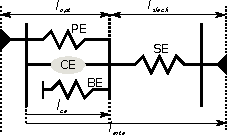
\includegraphics[scale=2.5]{figures/hill_muscle}
  \caption{Hill muscle model}
  \label{fig:hill_muscle}
\end{figure}

Where,

\begin{itemize}
\item $PE$ : Parallel element (Prevents muscle from over stretching)
\item $BE$ : Muscle Belly (Prevents muscle from collapsing on itself)
\item $SE$ : Series element or the muscle tendon element
\item $CE$ : Contractile Element or the active element
\item $l_{opt}$ : Muscle optimal fiber length
\item $l_{slack}$ : Muscle tendon slack length
\item $l_{CE}$ : Contractile element length
\item $l_{MTC}$ : Muscle Tendon Complex length
\end{itemize}


\begin{figure}[H]
  \centering
  \begin{subfigure}[b]{0.49\textwidth}
    { \centering
      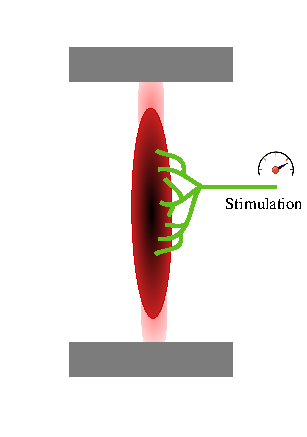
\includegraphics[width=\textwidth]{figures/isometric_muscle}
      \label{fig:isometric_muscle}
    }
    \caption{Isometric muscle setup :\\ To study the relationship
      between Force-Length.}
  \end{subfigure}
  \begin{subfigure}[b]{0.49\textwidth}
    { \centering
      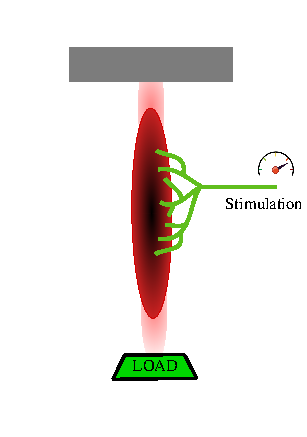
\includegraphics[width=\textwidth]{figures/isotonic_muscle}
      \label{fig:isotonic_muscle}
    }
    \caption{Isotonic muscle setup :\\ To study the relationship
      between Force-Velocity.}
  \end{subfigure}
  \caption{Muscle Length-Velocity-Force Setup}
  \label{fig:muscle-setup}
\end{figure}

\subsection*{Muscle Force-Length Relationship}
\label{sec:muscle-force-length}
In this exercise you will explore the relation between the length and
velocity of the muscle. In order to do this we replicate the set-up
show in figure \ref{fig:muscle-setup}.Here the length of the muscle is
held constant by attaching it's tendon to two fixed points. While
applying a constant stimulation, observing the force produced will
give the relationship between muscle contractile element length and
force.
\subsection*{2.a For a given stimulation, explore the relationship
  between active and passive muscle forces and the length of the
  contractile element.  Plot the force-length relationship curve.
  Discuss the different regions in the plot}

\subsection*{2.b In (2.a), you explored the muscle force-length
  relationship for a given stimulation. What happens to the
  relationship when the stimulation is varied between [0 - 1]? Support
  your response with relevant plots.}



\subsection*{2.c Describe how the fiber length ($l_{opt}$) influences
  the force-length curve.  (Compare a muscle comprised of short muscle
  fibers to a muscle comprised on long muscle fibers.)}

\subsection*{Muscle Velocity-Tension Relationship}
In this exercise you will explore the relation between the force and
velocity of the muscle. In order to do this we replicate the set-up
show in figure \ref{fig:muscle-setup}. Here the length of the muscle is
allowed to vary by attaching one of its end to a fixed point and the
other to a variable external load. While applying a constant load
initially and holding the muscle at constant length, a quick release
is performed to let the muscle contract and pull the weight. The
maximum velocity during this quick release will give us the
relationship between muscle contractile velocity and the force

\subsection*{2.d For a stimulation of 1.0 and starting at optimal
  muscle length, explore the relationship between contracticle element
  velocity and external load. Plot the Velocity-Tension relationship
  curve. Include shortening and lengthening regions}

\subsection*{2.e For the muscle force-velocity relationship, why is
  the lengthening force greater than the force output during
  shortening?}

\subsection*{2.f How does the parameter muscle activation influence the
  force-velocity relationship.  Show and explain the behavior for
  multiple muscle activation}

\end{document}

%%% Local Variables:
%%% mode: latex
%%% TeX-master: t
%%% End: